\documentclass{article}
\usepackage[utf8]{inputenc}
\usepackage{titlesec}
\usepackage{fullpage} % changes the margin
\usepackage{amsmath}
\usepackage{amssymb}
\usepackage{graphicx} %package to manage images
\usepackage[linkcolor=red]{hyperref}
\usepackage{paralist}
\usepackage{subcaption}
\usepackage{algpseudocode}
\usepackage{algorithm}
\usepackage{listings}
\usepackage{hyperref}
\usepackage{amsmath}
\usepackage{environ}
\usepackage{tabto,enumitem}
\usepackage{lipsum}
\usepackage{float}
\usepackage{tabto}
\usepackage{booktabs}
\graphicspath{ {./Image/} }

\title{Soen6011}
\author{Anushka }
\date{August 2022}
\title

\begin{document}
\begin{titlepage}
\vspace*{0.7in}
\begin{center}
\begin{figure}[htb]
\begin{center}

\includegraphics[width=8cm]{univ_logo}
\end{center}
\end{figure}
\vspace*{0.3in}
\begin{Large}
\textbf{SOEN 6011 : SOFTWARE ENGINEERING PROCESSES} \\
\end{Large}
\vspace*{0.1in}
\begin{Large}
\textbf{SUMMER 2022} \\
\end{Large}
\vspace*{0.9in}
\begin{Large}
\begin{center}
   \textbf{ Final Project - Function 7: \(x^y\)} \\ 
\end{center} 
\end{Large}
\vspace*{0.9in}
\begin{large}
Submitted To: Pankaj Kamthan \\
\vspace*{0.1in}

\date{\normalsize\today} 
\end{large}
\vspace*{0.1in}
\begin{large}
Submitted By: \\
\vspace*{0.1in}
Anushka Sharma\\
\vspace*{0.1in}
40159259\\
\vspace*{0.3in}
\date{\normalsize\today} 
\end{large}
\end{center}

\end{titlepage}
\tableofcontents
\newpage
\addcontentsline{toc}{section}{Problem 1 - a) Description of the function}
\section*{\centering{PROBLEM 1 - F7 : \(x^y\)}} 
\hfill Repository address : https://github.com/anush97/SOEN6011
\subsection*{Definition of \(x^y\)}
\cite{mathInsight} Exponentiation is a mathematical operation, denoted as \(x^y\), If y is a positive integer and \(x\) is any real number, then \(x^y\) corresponds to repeated multiplication.
 \begin{center} \(x^y\) = \(x\)*\(x\)*\(x\)*.....*\(x\) of y times \end{center}
The expression can be called as “\(x\) raised to the power of y,” “\(x\) to the power of y,” or simply “\(x\) to the y.” Here, \(x\) is the base and y is the exponent or the power.
\subsection*{Domain}
\cite{mathbits} All the real numbers from -infinite to +infinite.(-\(\infty\) to \(\infty\))
 \begin{center} $(x,y) \in \R^2 : (x \geq 0 \land y \neq 0) \lor x>0$ \end{center}
\subsection*{Co-domain}
A set of all positive real numbers from zero to infinite (0 to \(\infty\)) is known as the Exponentiation function
\begin{enumerate}
\item When y is a non-negative integer, the domain is all real numbers:  (- $\infty$,$\infty$)

\item When y is a negative integer, the domain is all real numbers excluding zero ( (- $\infty$, 0) $\cup$ (0,$\infty$) )

\item When y is an irrational number and y \textgreater \space 0, the domain is all non-negative real numbers and when y is an irrational number and y \textless \space 0, the domain is all positive real numbers

\item The co-domain of the function is [- $\infty$,$\infty$] and can be indeterminate
\end{enumerate}
\begin{flushleft}
\\\\
\textbf{Graph Characteristics}
 \end{flushleft}
\begin{flushleft}
\cite{mathbits}\cite{wolframalpha} The \textbf{rate of change} increases (or decreases) across the graph in an exponential graph.
\end{flushleft}
\begin{itemize}
\item \label{graph} The exponential graph crosses the y-axis at (0,1). 
\item The exponential graph increases, when x \(>\) 1.
\item The exponential graph decreases, when 0 \(<\) x \(<\) 1.
\item The exponential graph is asymptotic to the x-axis - gets very, very close to the x-axis but, in this case, does not touch it or cross it.
\end{itemize}
\begin{center}
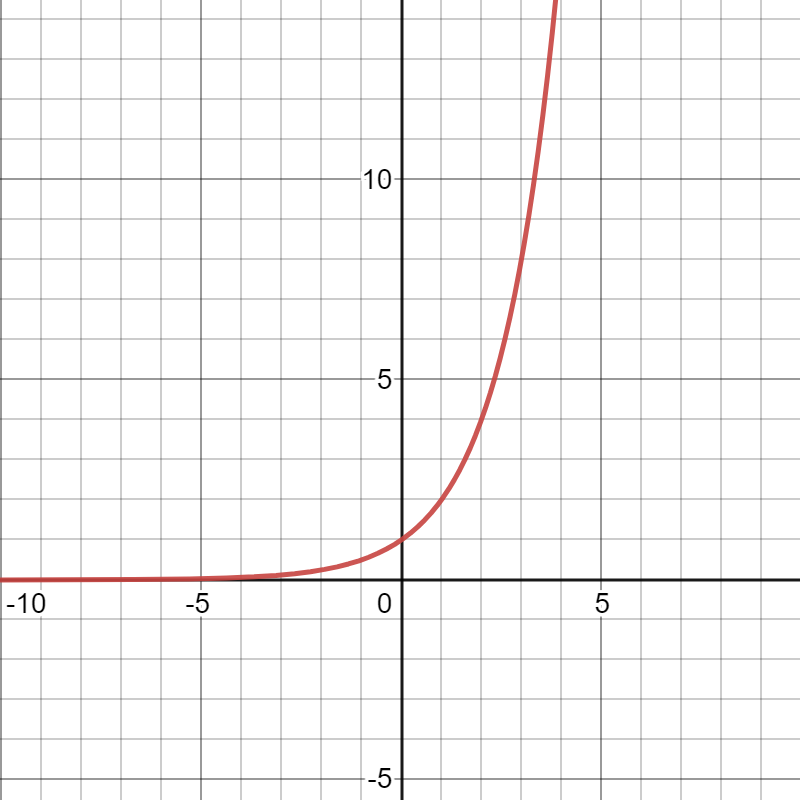
\includegraphics[width=5cm]{x^y}
\end{center}
\begin{center}
Graph crosses the y-axis at (0,1)\end{center}

\\
\addcontentsline{toc}{section}{Problem 1 - b) Context of Use Model}
\section*{b) Context of Use Model}
\normalsize{The users of the calculator shall be using it to calculate the result of function on two numbers. These numbers shall be an integer or decimal,so the valid inputs are the digits \textit{0-9} and the decimal points.The calculator should return the result or a message that indicates why it was unable to do so.}
\begin{center}
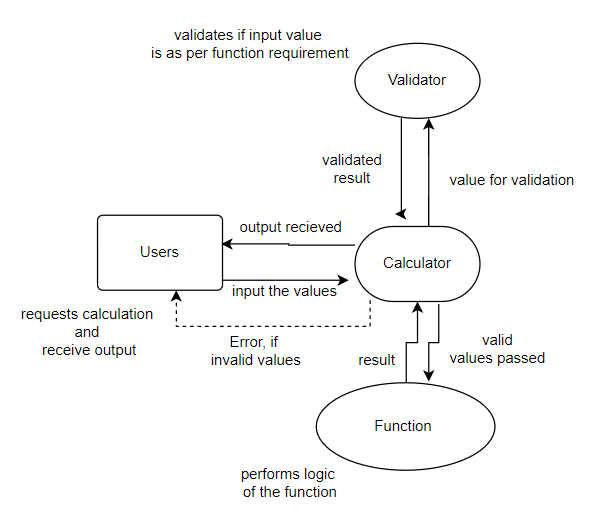
\includegraphics[width=15cm]{context}
\end{center}


\pagebreak
\addcontentsline{toc}{section}{Problem 2 - Requirements}
\section*{\centering{PROBLEM 2 - F7 : \(x^y\)}}
\section*{Requirements}\cite{ReqView}\cite{29148}\\
This section describes the requirements to implement the function 7 \(x^y\).
\\\\
\textbf{Assumption :} The transcendental function \(x^y\) will be accurate and accepts input which comprises of rational and irrational numbers.The exponential power will always be positive.
\\\\\\
\textbf{Requirement Id : F7-R1}\\\\
\begin{tabular}{ll}
\textbf{Overview} & X(0) to the power of Y(0) \\
\textbf{Version} & 1.0 \\
\textbf{Description} & 
\begin{tabular}[c]{@{}l@{}}If the user gives an input for X as Zero and input for Y as Zero.\\The function may return the 1 as output.
\end{tabular} \\
\textbf{Owner} & Anushka Sharma \\
\textbf{Priority} & High \\
\textbf{Type} & Functional \\
\textbf{Difficulty} & Medium \\
\textbf{Verification Method} & F7\_TC\\
\end{tabular}
\\\\\\\\
\textbf{Requirement Id : F7-R2}\\\\
\begin{tabular}{ll}
\textbf{Overview} & X(0) to the power of Y(Real Number) \\
\textbf{Version} & 1.0 \\
\textbf{Description} & 
\begin{tabular}[c]{@{}l@{}}If the user gives an input for X as zero and input for Y as
\\any Real Number. The function may return zero as output.
\end{tabular} \\
\textbf{Owner} & Anushka Sharma \\
\textbf{Priority} & High \\
\textbf{Type} & Functional \\
\textbf{Difficulty} & Medium \\
\textbf{Verification Method} & F7\_TC\\                                   \end{tabular}
\\\\\\\
\textbf{Requirement Id : F7-R3}\\\\
\begin{tabular}{ll}
\textbf{Overview} & X(Positive Number) to the power of Y(0) \\
\textbf{Version} & 1.0 \\
\textbf{Description} & 
\begin{tabular}[c]{@{}l@{}}If the user gives an input for X of any positive number and\\input for Y as Zero.The function may return 1 as the output.
\end{tabular} \\
\textbf{Owner} & Anushka Sharma \\
\textbf{Priority} & High \\
\textbf{Type} & Functional \\
\textbf{Difficulty} & Medium \\
\textbf{Verification Method} & F7\_TC\\                                                         \end{tabular}
\\\\\\\\
\textbf{Requirement Id : F7-R4}\\\\
\begin{tabular}{ll}
\textbf{Overview} & X(Negative Number) to the power of Y (0) \\
\textbf{Version} & 1.0 \\
\textbf{Description} & 
\begin{tabular}[c]{@{}l@{}}If the user gives an input for X of any negative number and
\\input for Y as Zero.The function may return 1 as the output.
\end{tabular} \\
\textbf{Owner} & Anushka Sharma \\
\textbf{Priority} & High \\
\textbf{Type} & Functional \\
\textbf{Difficulty} & Medium \\
\textbf{Verification Method} & F7\_TC\\
\end{tabular}
\\\\\\\\
\textbf{Requirement Id : F7-R5}\\\\
\begin{tabular}{ll}
\textbf{Overview} & X(Positive Number) to the power of Y(1) \\
\textbf{Version} & 1.0 \\
\textbf{Description} & 
\begin{tabular}[c]{@{}l@{}}If the user gives an input for X as any positive number and input \\for Y as 1. The function may return X as the output.
\end{tabular} \\
\textbf{Owner} & Anushka Sharma \\
\textbf{Priority} & High \\
\textbf{Type} & Functional \\
\textbf{Difficulty} & Medium \\
\textbf{Verification Method} & F7\_TC\\
\end{tabular}
\\\\\\\
\textbf{Requirement Id : F7-R6}\\\\
\begin{tabular}{ll}
\textbf{Overview} & X(Positive Number) to the power of Y(Positive Number) \\
\textbf{Version} & 1.0 \\
\textbf{Description} & \begin{tabular}[c]{@{}l@{}}If the user gives an input for X as any positive number and input \\for Y as positive number. The function may return positive \\number as the output.\end{tabular} \\
\textbf{Owner} & Anushka Sharma \\
\textbf{Priority} & High \\
\textbf{Type} & Functional \\
\textbf{Difficulty} & Medium \\
\textbf{Verification Method} & F7\_TC\\                                    \end{tabular}
\\\\\\
\textbf{Requirement Id : F7-R7}\\\\
\begin{tabular}{ll}
\textbf{Overview} & X(Negative Number) to the power of Y(Positive Even Number) \\
\textbf{Version} & 1.0 \\
\textbf{Description} & \begin{tabular}[c]{@{}l@{}}If the user gives an input for X as any Negative number and input \\for Y as positive Even number. The function may return positive \\number as the output.\end{tabular} \\
\textbf{Owner} & Anushka Sharma \\
\textbf{Priority} & High \\
\textbf{Type} & Functional \\
\textbf{Difficulty} & Medium \\
\textbf{Verification Method} & F7\_TC\\                                    \end{tabular}
\\\\\\\
\textbf{Requirement Id : F7-R8}\\\\
\begin{tabular}{ll}
\textbf{Overview} & X(Negative Number) to the power of Y(Positive Odd Number) \\
\textbf{Version} & 1.0 \\
\textbf{Description} & \begin{tabular}[c]{@{}l@{}}If the user gives an input for X as any negative number and input \\for Y as positive odd number. The function may return negative \\number as the output.\end{tabular} \\
\textbf{Owner} & Anushka Sharma \\
\textbf{Priority} & High \\
\textbf{Type} & Functional \\
\textbf{Difficulty} & Medium \\
\textbf{Verification Method} & F7\_TC\\                                    \end{tabular}


\pagebreak

\addcontentsline{toc}{section}{Problem 3 - Algorithms}
\section*{\centering{PROBLEM 3 - F7 : \(x^y\)}}
\textbf{\\ \\ Algorithm : Montgomery's Ladder Technique}\cite \\ 
\begin{itemize}
\item Montgomerym's ladder technique addresses defence against side-channel attacks for exponentiation computation. \\\\
The algorithm prevents the recovery of the exponent involved in the computation which could possibly benefit an attacker
\item The algorithm performs a fixed sequence of operations (up to log n): a multiplication and squaring takes place for each bit in the exponent, regardless of the bit's specific value.
\end{itemize}
\vspace*{0.2in}
\setlength{\tabcolsep}{18pt}
\renewcommand{\arraystretch}{1.5}
\begin{tabular}{ |p{6cm}|p{6cm}| }
\hline
\textbf{Advantages} & \textbf{Disadvantages}
\\ \hline 
It addresses the concern of MIM(Middle Man attack) observing the sequence of squaring and multiplications can (partially) recover the exponent involved in the computation. & Cache timing attacks are not yet protected and memory access latency might still be observable to an attacker\\
\hline
\end{tabular} 

\textbf{\\ \\ Algorithm : Taylor series}\\ \\Taylor series is a representation of a function as an infinite sum of terms that are calculated from the values of the function's derivatives at a single point.
\begin{equation} \label{evalpow}
x^y= e^{y\ln x}
\end{equation}
\ref{evalpow} evaluation of $x^y$. Here, e is a mathematical constant approximately equal to  2.71828
\begin{equation} \label{extaylor}
e^x = 1 + x/1! + x^2/2! + x^3/3! + ...... 
\end{equation}
\ref{extaylor} express $e^x$ using Taylor Series
\begin{equation} \label{altextaylore}
e^x = 1 + (x/1) (1 + (x/2) (1 + (x/3) (........) ) ) 
\end{equation}
\ref{altextaylore} The series \ref{extaylor} can be re-written as above
\begin{equation} \label{logtaylor}
log(1+x) = x-x^2/2 + x^3/3- ... 
\end{equation}
\ref{logtaylor} express ln x using Taylor Series\\ \\

\setlength{\tabcolsep}{18pt}
\renewcommand{\arraystretch}{1.5}
\begin{tabular}{ |p{6cm}|p{6cm}| }
\hline
\textbf{Advantages} & \textbf{Disadvantages}\\ \hline 
Very useful for derivations
 & Successive terms get very complex and hard to derive\\
\hline
Can be used to get theoretical error bounds &Truncation error tends to grow rapidly away from expansion point\\
\hline
Power series can be inverted to yield the inverse function & Almost always not as efficient as curve fitting or direct approximation\\
\hline
\end{tabular} \\ \\ 

\begin{algorithm}
\caption{Iterative algorithm to calculate $x^y$}
\begin{algorithmic}
\\ function \textbf{power\_function\_iterative(x,y)}\\
\textbf{in: } double number x,y\\
\textbf{out: } double number result
		\State $result \leftarrow 1$\\
   		 \State $temp \leftarrow 1$\\
for {$temp \leq y$} do\\
 \indent\qquad\State $result \leftarrow result*x$\\
 \indent\qquad\State $temp \leftarrow temp+1$\\
 end for \\
\State return result\\
\end{algorithmic}
\end{algorithm}

The output is stored in result, which is initially set to 1. It is then looped from 1 to y, x number of times, incremented by one on each iteration and on each iteration we multiply result by x. At the end of the loop value of result is equal to $x^y$.

\begin{algorithm}
\caption{Recursive Divide and Conquer algorithm to calculate $x^y$}
\begin{algorithmic} 
\\function \textbf{power\_function\_recursive(x,y)}\\
\textbf{in: } double number x,y\\
\textbf{out: } double number result
    \State $power \leftarrow exponent\_helper(x,y)$
    \State $result = power$\\
 return result
\end{algorithmic}
\end{algorithm}
\\
\begin{algorithm}
\begin{algorithmic}
\\1. function \textbf{exponent\_helper(x,y)}\\
\textbf{in: } double number x, y\\
\textbf{out: } double number sum\\
2. if  \State $x < 0$  then\\
3. \qquad $x \leftarrow 1.0 / x$ \\
4. \qquad $y \leftarrow -y$ \\
5. \qquad return $exponent\_helper(x,y)$ \\
6. else if \State $y = 0$ then \\
7.    \qquad return $1.0$ \\
8. else if  \StateE $y = 1$ then \\
9.    \qquad return x \\
10. else if  \State $y \mod  2 = 0$ then \\
11.    \qquad $y \leftarrow y * y$ \\
12.    \qquad $y \leftarrow y / 2$ \\
13.    \qquad return $exponent\_helper(x, y)$\\
14. else \\
15.    \qquad $x \leftarrow x * x$ \\
16.    \qquad $y \leftarrow y - 1$ \\
17.    \qquad $y \leftarrow y / 2$ \\
18.    \qquad return $exponent\_helper(x, y)$\\
19. end if \\
\end{algorithmic}
\end{algorithm}
A helper function called exponent\_helper is defined which calculates $x^y$. In the base case when $y = 0$, we return 1, otherwise when $y = 1$ we return x. When x is even we recurse on $x = x* x$ and $y = y /2$. In case when x is odd we recurse on $x = x* x$ and $y = (y-1)/ 2$. In the end, in our main function power\_function\_recursive we multiply the result of exponent\_helper to the value of a and return our result.
\subsection*{Advantages and Disadvantages}
\subsubsection*{Algorithm 1:}
Advantages:\\
1. In terms of space complexity, iterative algorithms don't suffer from stack overflow because all operations are done on the heap. \\
2. They are easy to comprehend by humans and have better readability.\\
Disadvantage:\\
1. The time complexity of the iterative algorithm is $O (n)$, hence it is not very efficient for larger inputs in terms of time.  \\
2. Proper terminating condition for loop is important or else it might lead to infinite looping.
\subsubsection*{Algorithm 2:}
Advantages: \\
1. The time complexity of the recursive algorithm is $O (log n)$. This recursive algorithm is optimized (tail recursive) so that we don't get stack overflow error and it handles large inputs better. \\
2. Recursion has higher maintainability than looping. Handling the base case properly requires little or no modifications.\\
Disadvantages:\\
1. Due to the continuous allocation of memory space leading to a stack overflow, efficiency is significantly affected. \\
2. It is difficult to comprehend. A certain level of expertise is required for understanding it vividly.\\
\subsubsection*{Conclusion}
Recursive algorithm which is based on Divide and Conquer Algorithmic Strategy is preferred over iterative algorithm due to above reasonings. \subsubsection*{Pseudocode Mind Map}
\begin{figure}[htb]
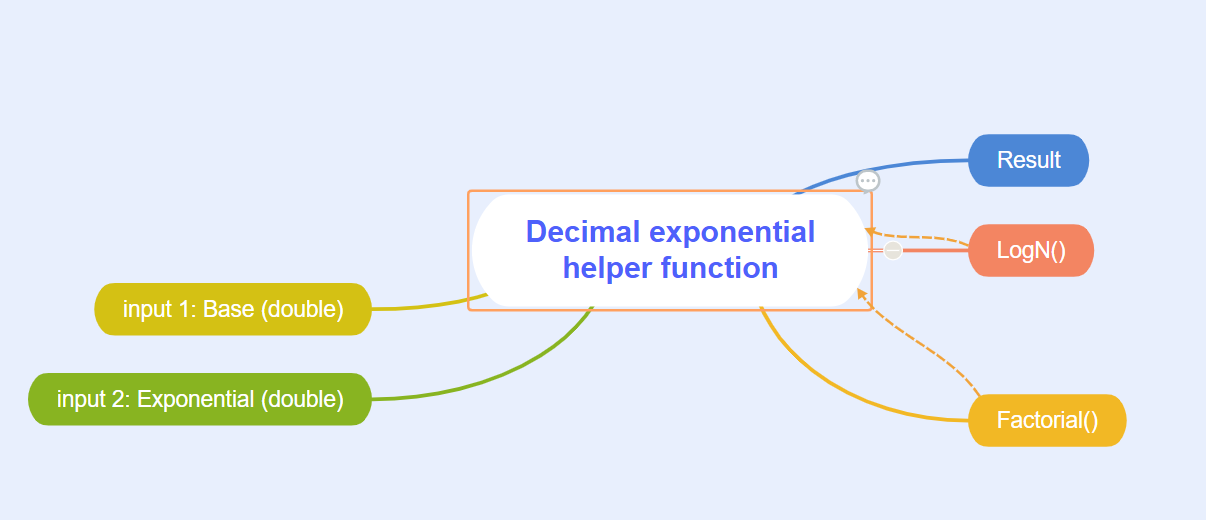
\includegraphics[width=12cm]{pseudo}
\centering
\caption{\textbf Mind Map of pseudocode}
\end{figure}
\pagebreak
\newpage
\addcontentsline{toc}{section}{Problem 4 - Source code Review of F7}
\section*{\centering{PROBLEM 4 - F7 : \(x^y\)}}
\section*{\textbf{Source code Review of F7}}
This section presents an overview of the source code of the Function 7 application \\(F7-Power Function)  and the
practices followed during the development.
\section*{Standard Programming Style used}
\begin{figure}[htp]
    \centering
    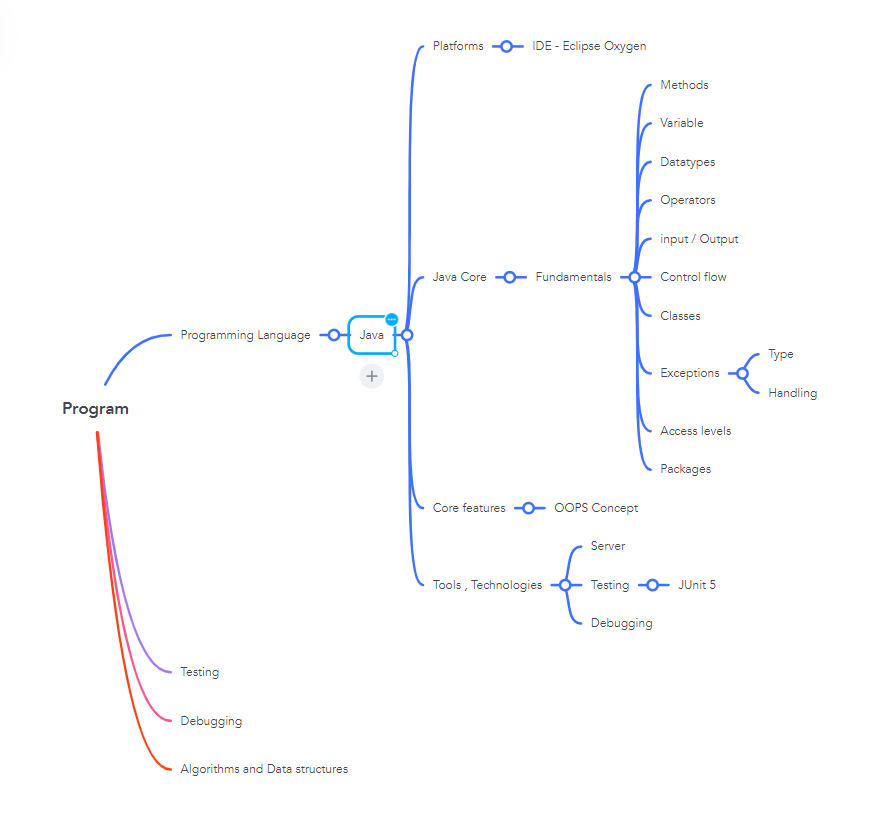
\includegraphics[width=17cm]{str-mindmap}
    \caption{Programming style Mind Map}
    \label{fig:galaxy}
\end{figure}
\subsection*{Naming Conventions}
The code satisfies to the google code style, and the method names and variable names in the code confirm to the standard of camel case nomenclature.
\newpage
\section*{Working of Source Code}
\begin{figure}[htp]
    \centering
    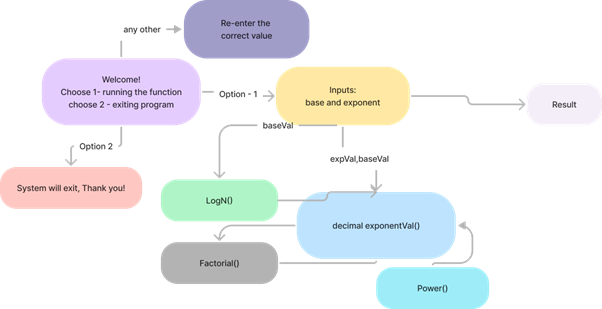
\includegraphics[width=10cm]{code-mindmap}
    \caption{Mindmap of code working}
    \label{fig:galaxy}
\end{figure}
\subsection*{JavaDoc}
Javadoc is added to facilitate the formation of highly readable documents and understanding of the code. They can define parameters, return type and authors like things for the methods of Classes and Objects.
\begin{figure}[htb]
    \centering
    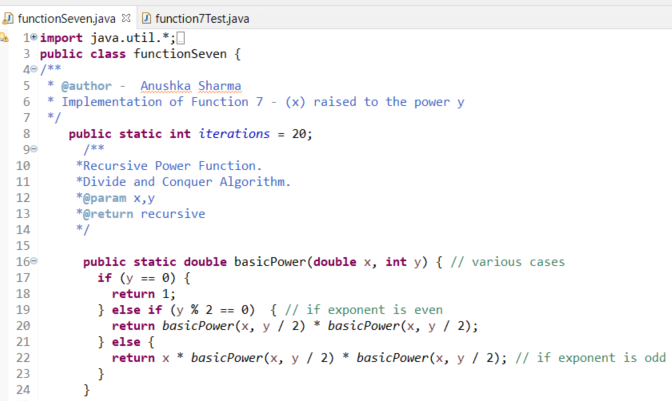
\includegraphics{javadoc}
    \caption{Javadoc in java file}
    \label{fig:galaxy}
\end{figure}
\newpage
\section*{Error Handling}
When an exception occurs, Its considered that the exception is thrown and it has to be caught.
When an exception is thrown, it is possible to "catch" the exception and prevent it from crashing the program. This is done with a try..catch block statement in the Function 7 as well. One can use many catch statements to handle various exceptions.
My main function consists of a try and catch block that is responsible for checking for an exception of NumberFormatException which is caused when the input in any of the base or exponent value is considered not double value or a value that cannot be converted into double. 
In simplified form, the syntax for a try..catch statement can be:
\begin{lstlisting}
try {
   statements-1
   ...
   numericInputCheck(inputDataString)
   ...
}
catch ( NumberFormatException exception) {
   statements-2
}
\end{lstlisting}
\begin{figure}[htb]
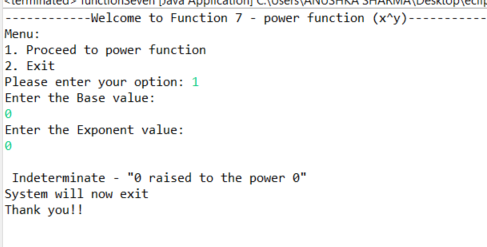
\includegraphics[width=0.6\textwidth]{Image/error.png}
\centering
\caption{ An Error message in the Function 7 that displays if the input is not accepted.
}
\end{figure}


\newpage
\section*{Debugger}
Eclipse has an in-built standard debugger allowing the program to open in a mode known as debug mode.Here, debugging can be performed step by step and we can also put break points so as to run just a section of the code.It offers multiple features like breakpoints , checkpoints and multiple views which enhance the experience of debugging.\\

\textbf{Advantages}

\begin{enumerate}
  \item Can add any variable that one want to monitor to watch list and see it working.\
  \item Eclipse debugger allows to remote debug a process on any other machine .\
  \item  The ability to execute code interactively—setting breakpoints, executing code line by line, and inspecting the value of variables and expressions.\
  \item The Eclipse Debugging Platform helps developers debug by providing buttons in the toolbar and key binding shortcuts to control program execution. \
\end{enumerate}

\textbf{Disadvantages}
\begin{enumerate}
\item Debugging with eclipse can be difficult if the execution of a particular function is time bound or if there is usage of thread or sleep statements within the file. \
\item For Multi threading, we have to use interfaces that themselves have their short comings . \\
\end{enumerate}
    \begin{figure}[htb]
    \centering
    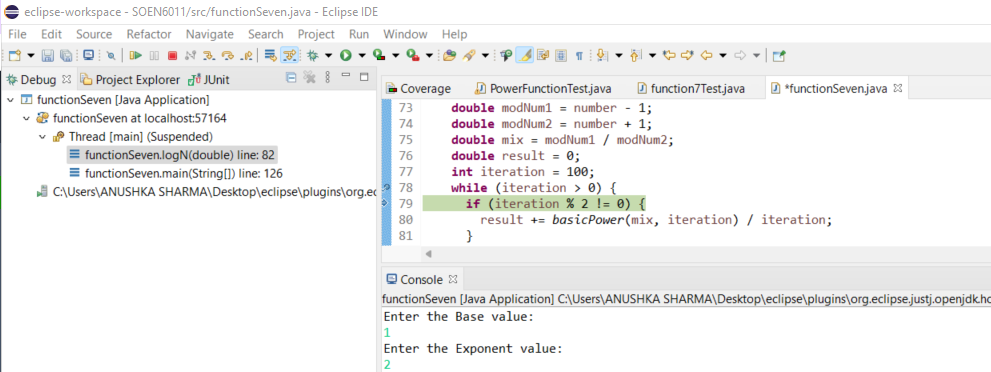
\includegraphics[width=16cm]{debug}
    \caption{Debugger of Eclipse.java}
    \label{fig:galaxy}
\end{figure}

\newpage
\subsection{Achieved Quality Attributes}


    \subsubsection{Space management}
        \begin{itemize}
            \item Limited variables are created
            \item Functions have been created to avoid duplicates of functionalities
            \item Used efficient methodology for the execution.
        \end{itemize}
        
    \subsubsection{Maintainability}
        \begin{itemize}
            \item Common practices has been adapted within a group to avoid ambiguities.
            \item Useful comments added in the code where it is required.
            \item Avoided global scoping for common variables and functions.
            \item Refactored code once every member merged their code to the github branch.
        \end{itemize}
    
   
    \subsubsection{Robustness}
        \begin{itemize}
            \item Usage of exception for exceptional test cases.
            \item Narrowed the variable scope as far as possible in the code.
            \item Error handling done on the code.
            \item Usage of mutable variable over creating new variables.
        \end{itemize}
  
    
    \subsubsection{Usable}
        \begin{itemize}
            \item Simple console interface provided for user input.
            \item Error messages are given in wrong input.
            \item Success messages are given for results.
            \item Suggestions are given when user encountered any difficulties while using calculator.
        \end{itemize}
        
    \subsubsection{Correctness}
        \begin{itemize}
            \item Coding standards is followed.
            \item Proper testing practices has been done on the function assigned. 
            \item JUnit Testing has implemented to check the correctness. 
        \end{itemize}
    \subsubsection{Efficiency}
    \begin{itemize}
        \item The main focus on readability is given to the code.4
        \item The program takes not less than two or three nanoseconds.
    \end{itemize}
    \newline
    \subsection{Quality Check of Source Code}
    It's a programming tool that automates the process of inspecting Java code as per the guidelines and standards, saving the time and effort of doing so manually. It's works well for projects that want to enforce a coding standard.
    \subsubsection*{Advantages}
    \begin{itemize}
        \item The checkstyle is portable between different IDEs.
        \item It can be easily integrated as a build tool into your Software Configuration Management i.e. projects.
        \item Checkstyle is a stand-alone framework, integrating it with your other tools is considerably easier as does not disturb the flow of the code.
    \end{itemize}
    \subsubsection*{Disadvantages}
    \begin{itemize}
        \item Checkstyle analyses one file at a time statistically.
    \end{itemize}
    \newline
\begin{figure}[htb]
    \centering
    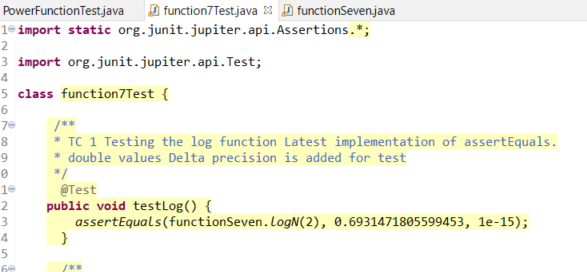
\includegraphics{checklist}
    \caption{Checkstyle of functionseven.java}
    \label{fig:galaxy}
\end{figure}
\pagebreak
\newpage
\addcontentsline{toc}{section}{Problem 5 - Unit Test Case Description}
\section*{\centering{PROBLEM 5 - F7 : \(x^y\)}}
\section*{\textbf{Unit Test Case Description}}
The unit test cases implemented using \textbf{JUnit5} for Function 7 (F7-Power Function) which are traceable to requirements in section 2.\\\\\\
\textbf{Test Case : F7\_TC\_1}\\\\
\begin{tabular}{ll}
\textbf{Test Case ID} & F7\_TC\_1 \\
\textbf{Requirement ID} & F7-R1 \\
\textbf{Action} & 
\begin{tabular}[c]{@{}l@{}}The user chooses "1 " to proceed with the function,\\ then input base value followed by exponential value and presses Enter. \\
\end{tabular} \\
\textbf{Input(s) } & base = 0.0, exponent = 0.0 \\
\textbf{Expected Output } & Indeterminate - "0 raised to the power 0" \\
\textbf{Actual Output } & Indeterminate - "0 raised to the power 0" \\
\textbf{Test Result } & Success \\
\end{tabular}
\\\\\\\\
\textbf{Test Case : F7\_TC\_2}\\\\
\begin{tabular}{ll}
\textbf{Test Case ID} & F7\_TC\_2 \\
\textbf{Requirement ID} & F7-R2 \\
\textbf{Action} & 
\begin{tabular}[c]{@{}l@{}}The user chooses "1 " to proceed with the function,\\ then input base value followed by exponential value and presses Enter. \\
\end{tabular} \\
\textbf{Input(s) } & base = 0.0, exponent = 6.0 \\
\textbf{Expected Output } & 0.0 \\
\textbf{Actual Output } & 0.0 \\
\textbf{Test Result } & Success \\
\end{tabular}
\\\\\\\\\
\textbf{Test Case : F7\_TC\_3}\\\\
\begin{tabular}{ll}
\textbf{Test Case ID} & F7\_TC\_3 \\
\textbf{Requirement ID} & F7-R3 \\
\textbf{Action} & 
\begin{tabular}[c]{@{}l@{}}The user chooses "1 " to proceed with the function,\\ then input base value followed by exponential value and presses Enter. \\
\end{tabular} \\
\textbf{Input(s) } & base = 37.0, exponent = 0.0 \\
\textbf{Expected Output } & 1.0 \\
\textbf{Actual Output } & 1.0 \\
\textbf{Test Result } & Success \\
\end{tabular}
\\\\\\\\
\textbf{Test Case : F7\_TC\_4}\\\\
\begin{tabular}{ll}
\textbf{Test Case ID} & F7\_TC\_4 \\
\textbf{Requirement ID} & F7-R4 \\
\textbf{Action} & 
\begin{tabular}[c]{@{}l@{}}The user chooses "1 " to proceed with the function,\\ then input base value followed by exponential value and presses Enter. \\
\end{tabular} \\
\textbf{Input(s) } & base = -9.0, exponent = 0.0 \\
\textbf{Expected Output } & 1.0 \\
\textbf{Actual Output } & 1.0 \\
\textbf{Test Result } & Success \\
\end{tabular}
\\\\\\\\
\textbf{Test Case : F7\_TC\_5}\\\\
\begin{tabular}{ll}
\textbf{Test Case ID} & F7\_TC\_5 \\
\textbf{Requirement ID} & F7-R5 \\
\textbf{Action} & 
\begin{tabular}[c]{@{}l@{}}The user chooses to proceed with the function , then input base value followed by exponential value and presses Enter.. \\
\end{tabular} \\
\textbf{Input(s) } & base = 7.0, exponent = 1.0 \\
\textbf{Expected Output } & 7.0 \\
\textbf{Actual Output } & 7.0 \\
\textbf{Test Result } & Success \\
\end{tabular}
\\\\\\\\\\\\
\textbf{Test Case : F7\_TC\_6}\\\\
\begin{tabular}{ll}
\textbf{Test Case ID} & F7\_TC\_6 \\
\textbf{Requirement ID} & F7-R6 \\
\textbf{Action} & 
\begin{tabular}[c]{@{}l@{}}The user chooses "1 " to proceed with the function,\\ then input base value followed by exponential value and presses Enter. \\
\end{tabular} \\
\textbf{Input(s) } & base = 5, exponent = 9 \\
\textbf{Expected Output } & 1953125.0 \\
\textbf{Actual Output } & 1953125.0 \\
\textbf{Test Result } & Success \\
\end{tabular}
\\\\\\\\
\textbf{Test Case : F7\_TC\_7}\\\\
\begin{tabular}{ll}
\textbf{Test Case ID} & F7\_TC\_7 \\
\textbf{Requirement ID} & F7-R6 \\
\textbf{Action} & 
\begin{tabular}[c]{@{}l@{}}The user chooses "1 " to proceed with the function,\\ then input base value followed by exponential value and presses Enter. \\
\end{tabular} \\
\textbf{Input(s) } & base = -3, exponent = 4.4     \\
\textbf{Expected Output } & 125.916 \\
\textbf{Actual Output } & 125.916 \\
\textbf{Test Result } & Success \\
\end{tabular}
\\\\\\
\textbf{Test Case : F7\_TC\_8}\\\\
\begin{tabular}{ll}
\textbf{Test Case ID} & F7\_TC\_8 \\
\textbf{Requirement ID} & F7-R6 \\
\textbf{Action} & 
\begin{tabular}[c]{@{}l@{}}The user chooses "1 " to proceed with the function,\\ then input base value followed by exponential value and presses Enter. \\
\end{tabular} \\
\textbf{Input(s) } & base = -9, exponent = 3 \\
\textbf{Expected Output } & -729 \\
\textbf{Actual Output } & -729 \\
\textbf{Test Result } & Success \\
\end{tabular}\\
Hence all the requirements were satisfied and all the test cases passed. Unit Test case report are as follows:\\
\begin{figure}[htb]
\begin{center}
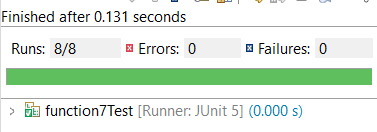
\includegraphics{coverage1}
\centering
  \caption{ Test case result of function F7 : \(x^y\)  using Junit4
}
\end{center}
\end{figure}
\begin{figure}[htb]
\begin{center}
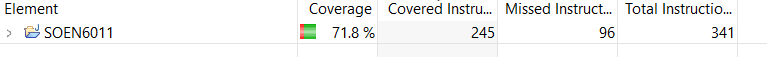
\includegraphics{coverage2}
\newline
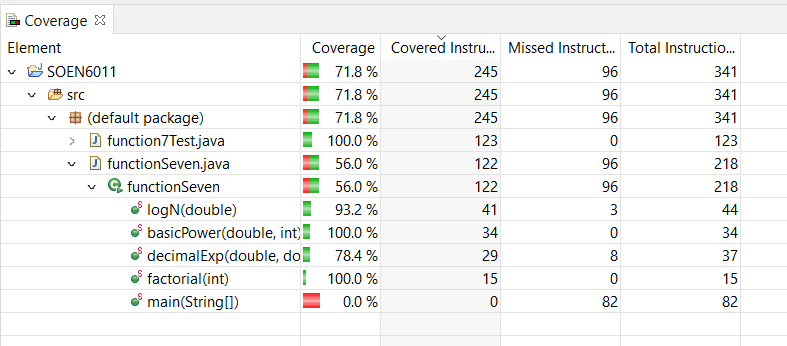
\includegraphics{coverage3}
  \centering
  \caption{ Coverage of JUnit testing of function F7 : \(x^y\)
}
\end{center}
\end{figure}
\pagebreak
\newpage

\begin{thebibliography}{}


\bibitem{mathInsight} 
Nykamp DQ: Basic rules for exponentiation
\\\texttt{https://mathbitsnotebook.com/Algebra2/Exponential/EXExpFunctions.html}
\bibitem{mathbits} 
MathBits Teacher: Exponential Functions,
\\\texttt{https://mathbitsnotebook.com/Algebra2/Exponential/EXExpFunctions.html}
\bibitem{wolframalpha} 
WolframAlpha: Domain of exponentiation function,
\\\texttt{https://www.wolframalpha.com/input/?i=x\%5Ey}
\bibitem{ReqView} 
ReqView : Nykamp DQ: Requirements Specification Templates
\\\texttt{https://www.reqview.com/doc/iso-iec-ieee-29148-templates}
\bibitem{29148} 
29148-2018-ISO/IEC/IEEE International Standard-Systems and software engineering-Life cycle processes-Requirements engineering,
\\\texttt{https://standards.ieee.org/standard/29148-2018.html}

\bibitem{CheckStyle} 
 CheckStyle. Eclipse Checkstyle Plugin. 2019.
\\\texttt{ https://checkstyle.org/eclipse-cs}

\bibitem{test1}
Mike Spivey. "The fuzz Manual" Manual and software copyright . J. M. Spivey 1988, 1992, 2000
\end{thebibliography}
\end{document}
